\begin{figure}[h!]
\textbf{Tema d'Esame di Gennaio 2017}\\ \\
Calcolare il periodo di un pendolo lungo $2 m$ a $50000 km$ dalla superficie della terra, sapendo che la massa e il raggio della terra sono $5.97\cdot 10^{24} kg$ e $6371 km $ rispettivamente.
\end{figure}

\begin{figure}[h!]
\textbf{Tema d'Esame di Febbraio 2017}\\ \\
 Il periodo di rotazione della luna intorno alla terra è $T_L = 27.32$ giorni e la sua orbita è approssimativamente circolare di raggio $d = 384400 km$. L’accelerazione di gravità sulla
superficie terrestre è $g = 9.81 m/s^2$
. Si valuti il raggio terrestre $r_T$ utilizzando esclusivamente i dati precedenti (non usare nemmeno la costante gravitazionale $G$).
\end{figure}

\begin{figure}[h!]
\textbf{Tema d'Esame di Luglio 2017}\\ \\
Sull'asse che unisce la terra con la luna (distanza terra-luna $D_{TL} =3.8\cdot 10^8 m$), a quale distanza dal centro della terra ($M_T = 6.0\cdot 10^{24} kg$) la forza gravitazionale netta esercitata su un corpo di massa $M$ è nulla? (massa Luna $M_L = 7.4\cdot 10^{22} kg$)
\end{figure}

\begin{figure}[h!]
\textbf{Tema d'Esame di Settembre 2017}\\ \\
Un sistema binario di stelle ruota circolarmente attorno al comune centro di massa a metà del segmento che le unisce. Ciò significa che la massa delle due stelle è uguale. Se la velocità orbitale di ciascuna di esse è $v = 220 km/s$ ed il
periodo orbitale di ciascuna è $14.4$ giorni, trovare la massa $M$ di ciascuna stella. 
\begin{center}
		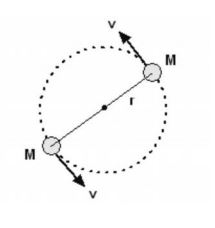
\includegraphics[scale=1]{ES3/SET032017.jpg}
\end{center}
\end{figure}